\chapter{Experimental Setup}
Two open-source controllers operating systems were compared. Ryu and Pox are installed on a server machine. In contrast, Mininet and CBench are installed on two different host machines in the following hardware and software configurations.

 \begin{table}[!hbt]
    \centering
    \caption{Features of Pox and Ryu}
    \begin{tabular}{|p{5cm}|p{5cm}|p{5cm}|}
    \hline
         \textbf{Features} & \textbf{Pox} & \textbf{Ryu} \\ \hline
         OpenFlow Version & v1.0 & v1.0, v1.2, v1.3, v1.4, v1.5, Niciria extensions \\ \hline
         GUI & Yes & Yes \\ \hline
         REST API & Yes & Yes \\ \hline
         Platform Support & Windows, Linux, Mac & Linux \\ \hline
    License Provider & Apache & Apache \\ \hline
    Learning Curve & Easy & Moderate \\ \hline
    Distributed Support & No & Yes \\ \hline
    Last Updated & Nov 2017 & May 2020 \\ \hline
    \end{tabular}
    \label{RyuvsPox}
    \end{table}
    
\section{Hardware Configuration}
    \begin{table}[!hbt]
    \centering
    \caption{Physical constraints of Server and Host Machines}
    \begin{tabular}{|c|c|}
    \hline
    Architecture & x86\_64 \\ \hline
         CPU op-mode(s) & 32-bit, 64-bit \\ \hline
         CPU(s) & 8 \\ \hline
         Thread(s) per core & 2 \\ \hline
         Vendor ID & GenuineIntel \\ \hline
    Model name & Intel(R) Core(TM) i7-4790K CPU @ 4.00GHz \\ \hline
    L1d cache & 128 KiB \\ \hline
    L1i cache & 128 KiB \\ \hline
    L2 cache & 1 MiB \\ \hline
    L3 cache & 8 MiB \\ \hline
    \end{tabular}
    \label{Hardware}
    \end{table}

The configurations, as mentioned above, were not voluntarily chosen; rather, it was the resource restrictions during the project's time. Nevertheless, these configurations could be further modified based on repeated tests. So, even the worst-performing controller is best considering the limited processing power and RAM.

\section{Software \& Tools}
The controller is run on a Linux Ubuntu Server 18.04 LTS OS so that it got dedicated RAM and processor cores \cite{resshare1970}, and 5 out of 8 cores were isolated for the controller using \textit{isolcpus} tool.

Perf was also installed along with the controllers on the server machine itself but on a different single isolated core to prevent influence from any other running process(s).

Oracle VM VirtualBox is installed on two separate host machines. An instance of Linux Ubuntu Desktop 16.04.02 LTS OS is created.

Mininet is installed on the Host OS and is used to set the hosts, switches, controllers, and set any possible combinations of connections.

CBench tool emulates a set of switches and hosts per switch and connects to the SDN controller specified. Usually, it generates packets in the network and measures the performance of the controller in 2 modes
    \begin{itemize}
        \item Latency Mode: Packets in these events come in bulk from each switch.
        \item Throughput Mode: Packets in events come in sequential order.
    \end{itemize}

\begin{figure}[!hbt]
    \centering
        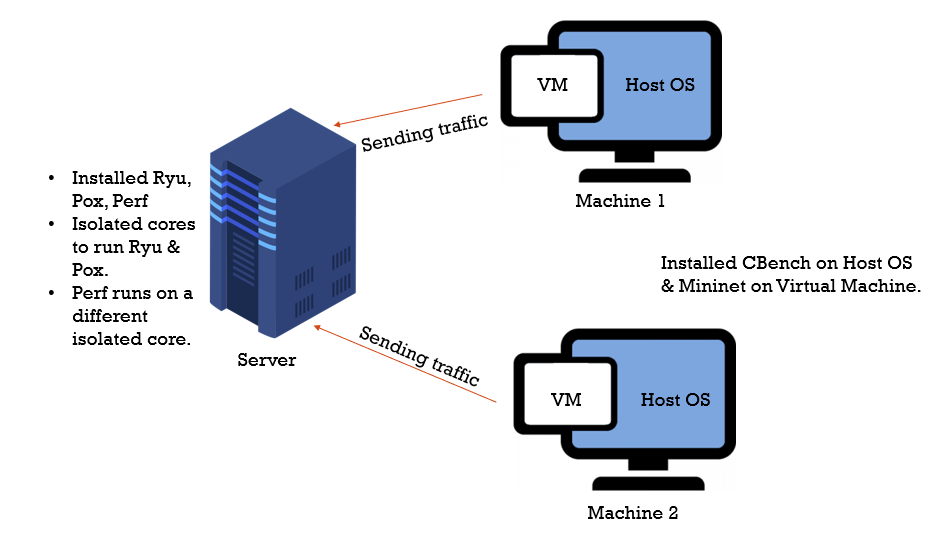
\includegraphics[width=\textwidth,keepaspectratio]{images/setup.png}
       \caption{Experimental Setup}
        \label{experimentalsetup}
\end{figure}

\begin{figure}[!hbt]
    \centering
        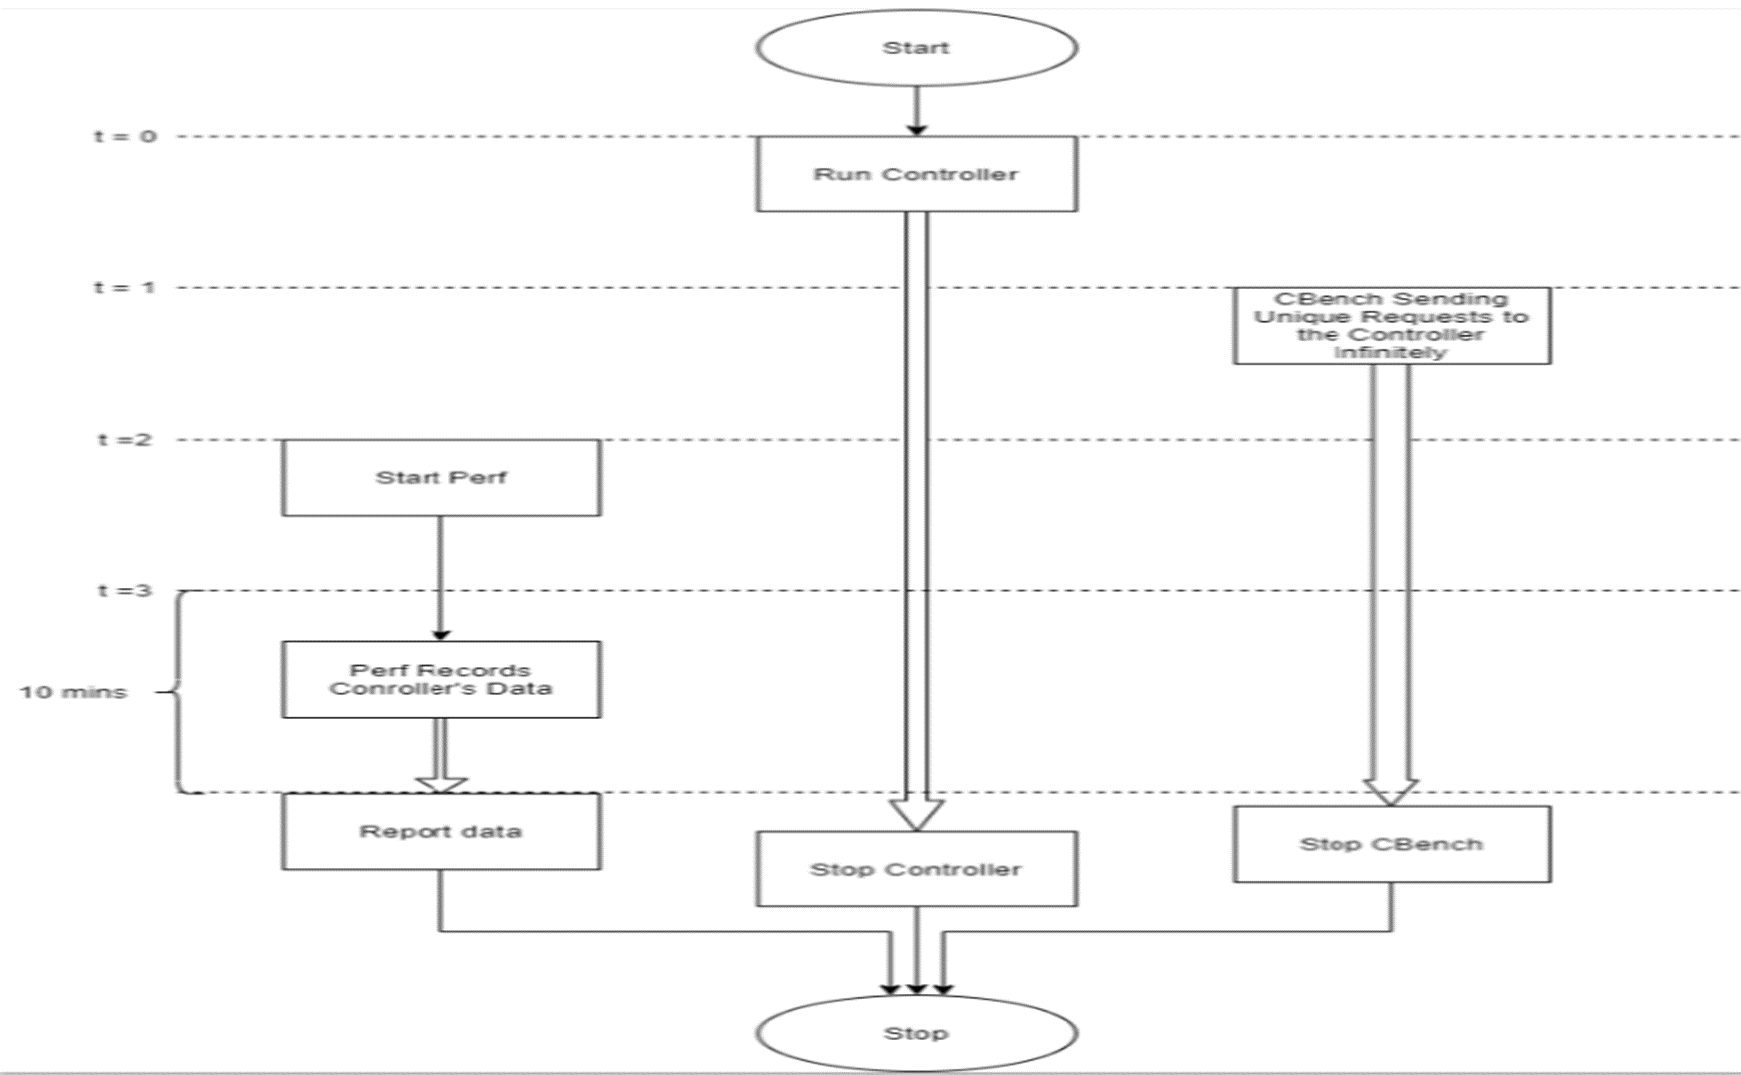
\includegraphics[width=\textwidth,keepaspectratio]{images/Workflow.PNG}
       \caption{Workflow of the Experiment}
        \label{workflowexperiment}
\end{figure}

However, in our case, we took the usage of CBench in throughput mode and generated massive traffic for the controller.

The overall experimental setup can be viewed as in Fig. \ref{experimentalsetup}

The experiment is carried on as the per the workflow, depicted in the Fig. \ref{workflowexperiment}